\chapter{Literature Review}\label{C:review}
In this chapter, we first introduce the background knowledge of web service composition in Subsection \ref{service} and \ref{servicecomposition}, i.e., properties of web service and web service composition, and service discover mechanisms. Second, EC techniques are also briefly introduced in Subsection \ref{ec}. Followed that Section \ref{related} reviews the single-objective service composition using EC and non-EC based techniques in Subsection \ref{singleobjective}.  Subsection  \ref{multiobjective} reviews existing works on multi-objective approaches and many-objective approaches.  Dynamic web service composition is covered in Subsection \ref{dynamicserivce}. Subsection \ref{Semantic}  discussed semantic service composition based on preconditions and effects. Lastly, Subsection \ref{summary} summarizes some key reviews and limitations in the literature review.
\section{Background}\label{background}
\subsection{Web Service}\label{service}
%We first introduce the concept of web services and a formal model from \cite{agarwal2010d5}, where both the functional and non-functional attributes are captured uniformly. Further, A Labelled Transition System \cite{agarwal2009making} is addressed with its abstract and updated model for demonstrating the behaviors of web services in Subsection \ref{functional}, which emphasizes on side of the functional attributes. After demonstrating these models, we will discuss about the nonfunctional properties of web services in Subsection \ref{nonfunctional}. Apart from these, we will discuss three main service discover mechanisms in \ref{servicediscovery}.

Web services are self-describing modules offering functionalities over the internet. The idea of web services is to allow customers to use them without prior specific knowledge. The functionalities of web services are often specified by their functional attributes, which satisfy users' functional requirements and provide mechanisms to allow users to search desired service. Web services are classified into two groups based on their functionalities:  \emph{information-providing services} and \emph{world-altering services} \cite{mcilraith2001semantic}. The first type of services expect some data returned by giving inputs or nothing. For example, an air velocity transducer web service reads the wind speed and returns the velocity at the time. This service does not require any inputs. On the other side, a city weather web service requires a city name and returns weather information for that city. Information-providing services do not produce any side effect to the world. The functionalities of these services are only inputs and outputs. The second type of services not only provide data information but also alters the status of the world by producing side effects. For example, a PayPal service will cause a deduction in the balance of users' bank account. \emph{In this proposal, we mainly focus the first type of services for first three objective. Later on, an extensive study is optionally carried for the second type of services}

As demonstrated above, the functional attributes determine what service really does, while the non-functional attributes often refers to some quality criteria, which is considered for raking services \cite{agarwal2009making}. In realistic scenarios, the non-functional are also important. For example, users may not prefer a service with higher cost with the same functionality provided by another one. Herein we will demonstrate both the functional and non-functional properties in following subsections.

%\emph{A Formal Model of Web Service} is demonstrated here: given a finite set $\wp$ of property types of web services and a finite set $\vartheta$ of values sets. Each property type is associated with a value set. We view a Web service as a finite set $Q$ of property instances with each property instance $q \in Q$ being of a property type$t(q) \in \wp$ that is associated with a value $v_q \in \vartheta_{t(q)}$. See Fig. \ref{fig:ws}

%\begin{figure}
%\centerline{
%\fbox{
%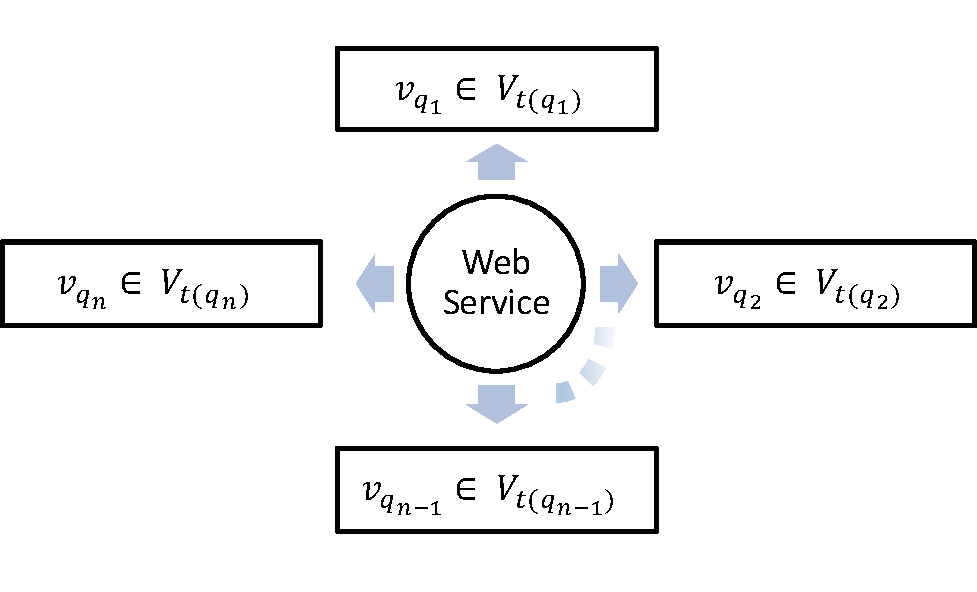
\includegraphics[width=8cm]{ws.pdf}
%}}
%\caption{Property-Based Web Service Formal Model \cite{agarwal2010d5}.}
%\label{fig:ws}
%\end{figure}

\subsubsection{Functional Properties of Web services}\label{functional}

%\emph{A Functionality Model} is demonstrated for describing all the functionalities of  web service. This mode is represented as a Labelled Transition System (LTS): $L = (S,T,\rightarrow)$ comprises a set $S$ of states, a set $T$ of transition labels and a labeled transition relation $\rightarrow \subseteq S \times T \times S$. This transition system is established to present the actual behavior of web services, which consists of a series of states. See Fig. \ref{fig:lts}.

%\begin{figure}
%\centerline{
%\fbox{
%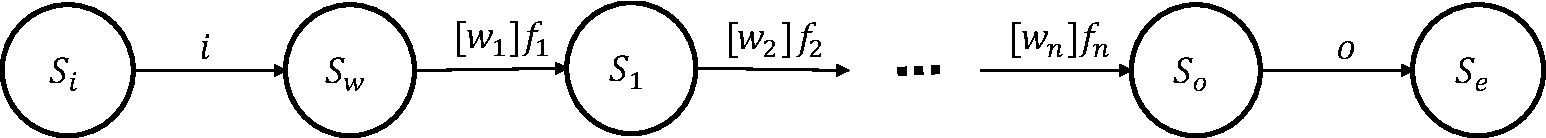
\includegraphics[width=14cm]{LTS.pdf}
%}}
%\caption{ The functionality of a Web Service \cite{agarwal2010d5}.}
%\label{fig:lts}
%\end{figure}
%
%\begin{itemize}
%\item $S_i$ start state includes knowledge available to web service before the web service is invoked by inputs; 
%\item $S_w$ state includes the inputs additional to the knowledge in 1; 
%\item A series of state $S_1$ to $S_n$ proceed with corresponding actions $f_n$ that only occurred if each related condition $[w_i]$ is approved to be true. 
%\item $S_o$ state contains all the outputs and all the changes performed in the knowledge base. 
%\item $S_e$ is the end state, which is equivalent to $S_o$, since the knowledge base is not changed.
%\end{itemize}

%The first functionality model presented above is not completely demonstrated for the internal actions, as the services provider does not want reveal all the internal functions, and it is not feasible to list a global set of property name. Therefore, \emph{An Abstract Functionality Model} is modeled by eliminating all the intermediate properties. In the abstract model of a web service, the functional properties of the web service could be identified as inputs $i$, pre-state $S_i$, outputs $o$ and post-state $S_o$. These four properties are mapped to a set of input $I$, preconditions $\phi$, a set of outputs $O$ and effects $\varphi$ respectively in third updated functionality model demonstrated below.
The operational characteristics of web services are related to the functional properties, which demonstrate the behaviors of web services, i.e., how services can be successfully invoked and what information are returned after execution. In other words, a set of inputs $I$ is required by a service and a set of output $O$ is returned by a service. For semantic web services, ontology reasoner is employed to reason about the properties (i.e., inputs and outputs) of web services, where a knowledge base is created to better enable the interoperability of the functional properties. Sometimes, the preconditions $\phi$ must be hold in the knowledge base before service execution, and they must remain consistent before passing the input $I$. Side effects are also created as effects $\varphi$ along with outputs $O$. All functional properties of web services are demonstrated in Fig. \ref{fig:ws}.


\begin{figure}
\centerline{
\fbox{
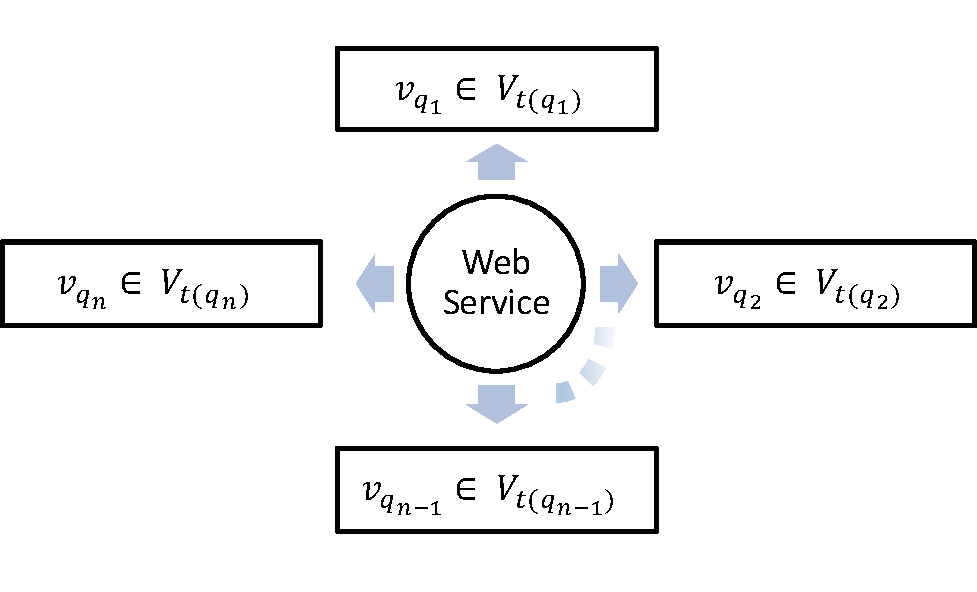
\includegraphics[width=8cm]{ws.pdf}
}}
\caption{Functional Properties of a Web Service.}
\label{fig:ws}
\end{figure}


%Apart from that, the precondition $\phi$ must be hold in the knowledge base before service is invoked by passing the input $I$. To enable the interoperability of the functional properties, ontology reasoner is employed to reason about the properties of web services. To distinguish the changes between before and after service execution, these changes are modeled as property instances. For example, inputs and outputs assigned as variable names and further referenced in preconditions and effects, which can be distinguished as different instances from the knowledge base. In particular, preconditions is assigned to the description of requirements of inputs using logic formula. Herein the description of the formula considers the following cases that are demonstrated using Planning Domain Description Language (PDDL \cite{fox2003pddl2}):
%\begin{itemize}
%\item Conditions on the type of inputs, e.g., the payment of an online shopping website is made by Visa or Cash: $\phi:(Format(payment)=Visa \cup Format(payment)=Cash)$.
%\item Relationships among inputs, e.g.,  authoried users are required for an online shopping: $\phi:(Authoried ? Useraccount)$.
%\item Conditions on the value of inputs, e.g., saving account balance has more than 100 dollars: $\phi: (\geq (amounts, saving account), 100)$
%\end{itemize}
%These preconditions must be hold in the state consistently while inputs are being passed to services. Similarly, the effects is restricted to the description of constraints on returned outputs, relationships between inputs and outputs, and changes caused by the service in the knowledge bases.

\subsubsection{Nonfunctional Properties of Web services}\label{nonfunctional}
Apart from the functional properties of web services discussed above, the non-functional properties of web services play an important part in composing services and often refer to QoS. For example, customers prefer lowest execution cost with highest response time and reliability. According to \cite{zeng2003quality}, four most often considered QoS parameters are as follows:
\begin{itemize}
\item \textit{Response time} ($T$) measures the expected delay in seconds between the moment when a request is sent and the moment when the results are received.
\item \textit{Cost} ($C$) is the amount of money that a service requester has to pay for executing the web service
\item \textit{Reliability} ($R$) is the probability that a request is correctly responded within the maximum expected time frame.
\item \textit{Availability} ($A$) is the probability that a web service is accessible.
\end{itemize}

\subsubsection{Web Service Discovery}\label{servicediscovery}
To generate service compositions, web service must provide mechanisms for discovery required services. Therefore, service discovery becomes a fundamental technique to be considered in all service composition approaches. \cite{agarwal2009d5} discussed three mechanisms of semantic web service discovery: classification-based approach, functionality-based approach and hybrid approach. Those service discovery techniques are further demonstrated below.

The first service discovery technique makes use of the classes provided by service semantic annotation in WSMO-Lite language. Therefore, service requesters can use class names to express a goal, which is a straightforward discovery from a set of classes. However, classes without clear meaning definition could lead to the issue of incomprehensibility of web service discovery. For example, several classes may declared in either different terms for the describing the same content or same terms for describing different content.

The second service discovery technique  does not take classes into account, but consider functional properties of web service to include pre-conditions and effects. In particular, a desired functionality description is defined. A discovery algorithm must be developed to handle a matching for different input, output, precondition and effects with associated concepts and relations in the provided domain knowledge base. The key idea of the matchmaking is to check whether services accept all the desired inputs provided by users and whether the desired outputs is delivered by services. In addition, this discovery technique also checks for the satisfiability of implications that actual precondition and actual effects must imply the desired precondition and desired effects respectively. The strength of the second is that it potentially meet the demands of all the comprehensible discovery, while the weakness is a lack of efficiency and scalability. 

The third service discovery technique is based on a hybridization of classification and functionality-based discovery. Classification hierarchy is proposed to achieve automatic semantic reasoning in hierarchical functionality. For example, a functionality class is associated with super classes and sub classes for more general functionality class and more specific functionality class respectively. However, to make a consistency of classification hierarchy, the inputs, outputs, precondition and effects of a functionality class must satisfy the conditions that contains all the inputs, outputs, precondition and effects of all the classes it is subsumed by. The advantage of this approach is to achieve better performance combining strengths of the previous two pure classifications based and functionality based approaches. While the classification hierarchy needs to be kept consistent when a new web service is published or updated.​

As discussed above, the first and third approach is considered either less effective or demands to build up a consistent ontology for classes and their functional attributes. It is not the focus of our research to build up any ontology for supporting classes or properties.  \emph{In the proposal, we use the second service discovery technique for meeting a comprehensible discovery. That is, different types of ontology reasoning are utilized to approach the matchmaking as a fundamental part of service composition algorithm.}



\subsection{Web Service Composition}\label{servicecomposition}

Since an atomic web service could not satisfy or fully satisfy users' complex functional requirements, web service composition is approached by composing web services together to meet the requirements. Manual service composition is very time-consuming and less productive. Therefore, many approaches have been developed to achieve semi-automated or fully automated service composition. The semi-automated service composition is inspired by the business process that required prior knowledge to build up abstract workflows. These workflows consist of abstract services, each of which is defined by input-output pairs. The details of these steps are further discussed in Subsection \ref{lifecycle}. On the other hand, when we are composing services, the interoperability of services is very important in both semi-automated and fully automated web service composition. In particular, several problems are simultaneously taken into account. That is I/O matchmaking (i.e., a mechanism for ensuring the interoperability ), discovery relevant services to the optimizing the quality of service composition, e.g., overall QoS. Consequently, the following concerns are required to consider in generating composition solution. 


\subsubsection{Web Service Composition Lifecycle}\label{lifecycle}
Typical steps in a workflow-based automated Web service composition solution are shown in Fig. \ref{fig:lifecycle}. The detail of the service lifecycle is discussed as follows:

\begin{figure}
\centerline{
\fbox{
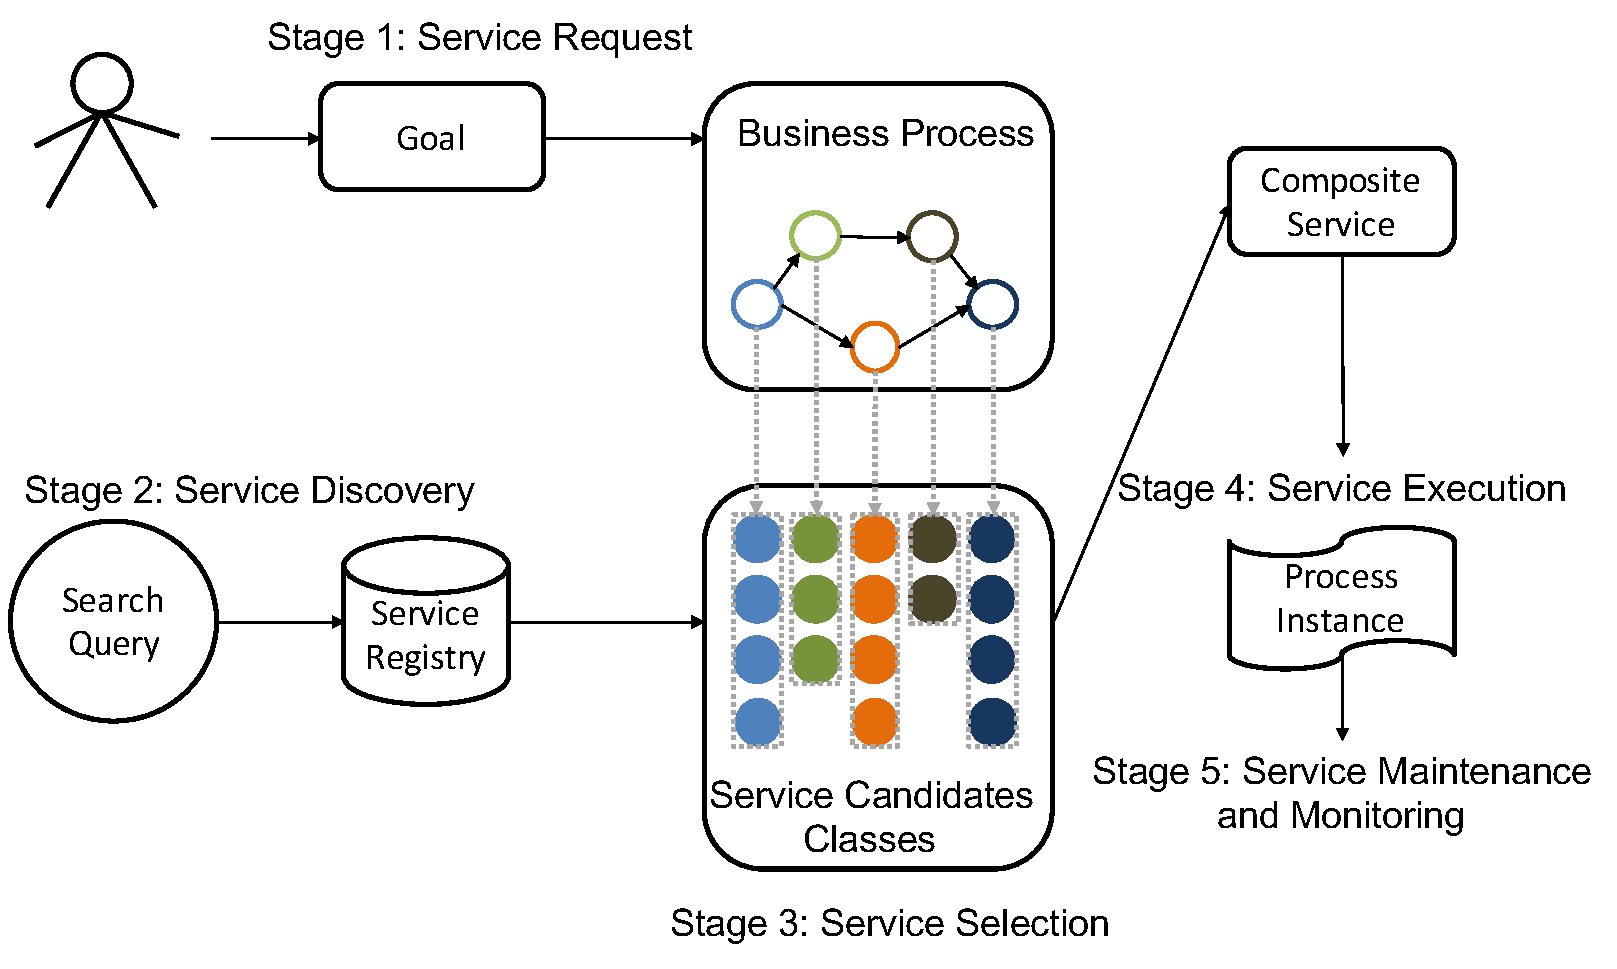
\includegraphics[width=14cm]{compositionLifecycle.pdf}
}}
\caption{ Web service composition lifecycle \cite{moghaddam2014service}.}
\label{fig:lifecycle}
\end{figure}

\begin{enumerate}
 \item \textit{Goal specification:} The first step in service composition is to collect users' requirements for composition goal that comprises of the functional (i.e., correct data flow ) and non-functional side (i.e., QoS). This step is achieved by building up an abstract workflow including a series of tasks with clearly defined functionalities. Those tasks could be completed by selecting proper concrete services to reach desired QoS. 
 \item \textit{Service discovery:} Once the goal is clearly specified, concrete web services will be selected for each task regarding its functional requirement. Often, more than one concrete web service is likely to be found to match one service discovery task. However, those matched web services are always different in QoS.
 \item \textit{Service selection:} At this stage, many techniques have been studied to select web services to best match each task for the satisfying functional requirement of each task and overall business process. Therefore, a plan of service composition is created ahead of execution.
 \item \textit{Service execution:} the process instance is monitored for any changes or services failures during service execution. In this stage, some actions are to be taken for adapting the changes.
\end{enumerate}
The web service lifecycle discussed above is a typical \emph{semi-automated approach}. There is a distinction between semi-automated and fully automated approaches. On the one hand, during the goal specification stage of semi-automated approach, the abstract workflow is already provided. An abstract workflow is not provided at the stage of goal specification for \emph{fully automated service composition}. Often, fully automated service composition rely on some algorithms (e.g., Graphplan algorithm \cite{blum1997fast}) to achieve service composition. Service workflow is gradually built up along with service discovery and service selection. In our thesis, I concentrate on developing methods for fully automated service composition, where service discovery and service selection are considered as interrelated tasks that are interleaved with the composition algorithm. 

\subsubsection{An Example of web service composition}
Fig. \ref{fig:wsc_example} shows a popular web service composition example from a travel domain. In this scenario, the agency provides customers a serial of services to satisfy their complex requirements. These services include flight bookings, accommodation reservations, bus services and map generations. In Fig. \ref{fig:wsc_example}, the task inputs (i.e., $TravelDepartureDate$, $TravelReturnDate$, $HomeCity$ and $ConferenceCity$ ) are gathered from customers, and task outputs (i.e., $BusTicket$, $FlightTicket$, $HotelReservation$ and $StreepMap$) are expected to be returned. Apart from those, the inputs of all the component services must be satisfied. In this example, we begin by executing the FlightBooking Service and GenerateMap Service, the FilightInformation service books the flights and determines a $arrivalDate$. Then, we use the $arrivalDate$ together with the other given data, we can book the hotel and bus, and generate Map for conference city. Together, these four services produce all required outputs for customers.

\begin{figure}
\centerline{
\fbox{
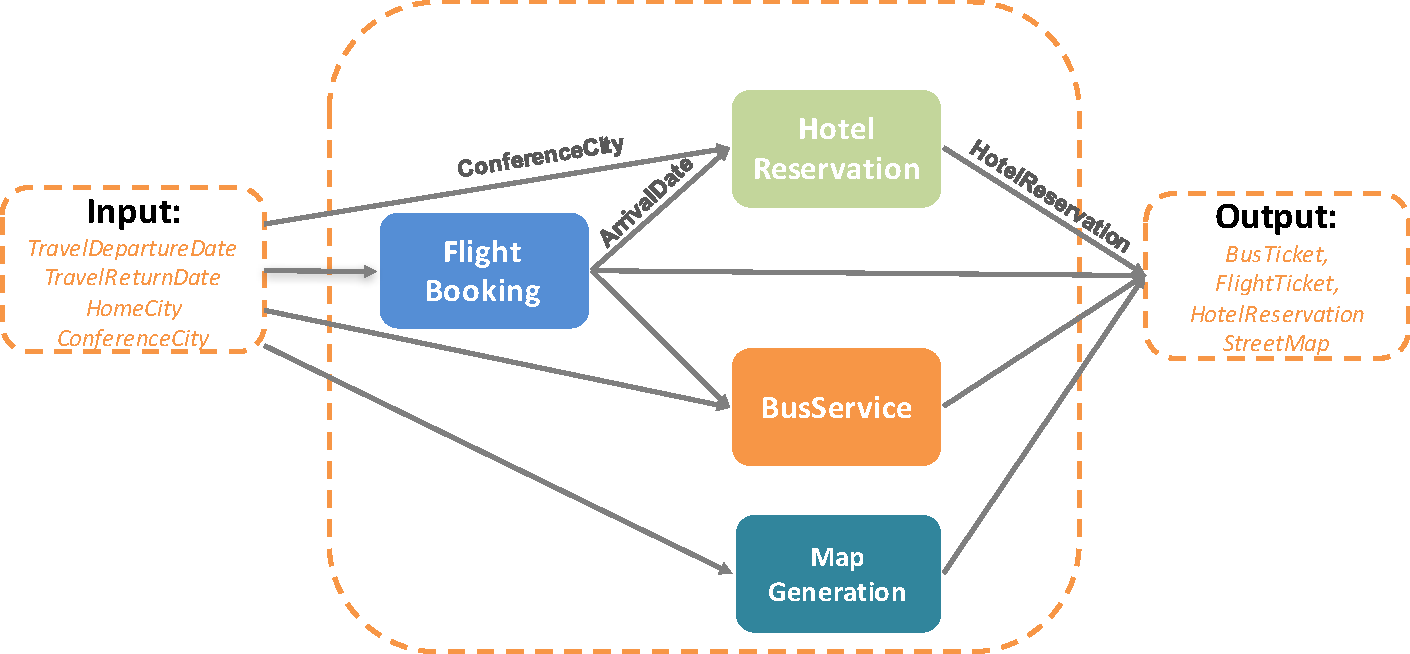
\includegraphics[width=14cm]{wsc_example.pdf}
}}
\caption{An example of traveling agency service.}
\label{fig:wsc_example}
\end{figure}

\subsubsection{Functional Properties of Web Service Composition}
From the example demonstrated above, two characteristics are addressed for the functional attributes of web service composition. One is that all the inputs of component services must be matched by given task inputs or produced outputs, so that service composition can be successfully executed. Another is that users' required inputs must be a subset of all the outputs of component web services, so that a service composition goal is successfully completed. 

In the first characteristics, often, the given task inputs or produced outputs often do not perfectly match the required services' inputs. For example, one component service from previous service composition example is pick up for further demonstration regarding the semantic matchmaking quality of the required inputs. The generateMap service requires inputs $MappedLocation$ and producing output $StreetMap$. Given that $instance-of (ConferenceCity,City)$, $instance-of (MappedLocation, Location)$ and $City \sqsubseteq Location$. We can see that $ConferenceCity$ is less preferable. Therefore, Semantic matchmaking quality between ConferenceCity and  MappedLocation is relatively lower. 

\begin{figure}
\centerline{
\fbox{

\includegraphics[width=14cm]{sm_example.pdf}
}}
\caption{An example for demonstrating semantic matchmaking quality.}
\label{fig:sm_example}
\end{figure}

Description logic (DL) makes it possible to measure the quality of semantic matchmaking. Substantial work \cite{bansal2016generalized,lecue2009optimizing, lecue2007making, lecue2006formal, rao2005semantic} utilizes Description logic (DL) reasoning between input and output parameters of web services for matchmaking, where different matchmaking types are considered for matchmaking, and they usually result in \emph{different matchmaking quality}. Therefore, exploring a effective mechanism for measuring the quality of semantic matchmaking in service composition is one of crucial tasks in our thesis. 

Firstly, we demonstrate different \emph{Matchmaking Types} discussed above here. Given two concepts $a, b$ in ontology $\mathcal{O}$, four commonly used matchmaking types are often used to describe the level of a match between outputs and inputs \cite{paolucci2002semantic}: 
\begin{itemize}
\item $exact$ returned, if $a$ and $b$ are equivalent ($a \equiv b$), 
\item $plugin$ returned, if $a$ is a sub-concept of $b$ ($a \sqsubseteq b$),
\item $subsume$ returned, if $a$ is a super-concept of $b$ ($a \sqsupseteq b$), 
\item $fail$ returned, if none of previous matchmaking types is returned. 
\end{itemize}

%Often, the similarity of two instances of two knowledge representations encoded in the same ontology is also
Secondly, to our best knowledge, three methods  \cite{lecue2007making, pop2009immune,shet2012new} are utilized for measuring the quality of semantic matchmaking in the domain of service composition. We will demonstrate these three methods below.

The first method measures the quality of matchmaking regarding the different matchmaking types. In \cite{lecue2007making}, the quality of semantic matchmaking is measured by the two quality criterion, matchmaking types and common description rate. They additionally consider $interaction$ matchmaking type ($a \sqcap b$), i.e., if the intersection of $a$ and $b$ is satisfiable. In their work, a causal link \begin{math} sl_{i,j} \stackrel{.}{=} \langle S_i, Sim_{T}(Out\_s_i,In\_s_j),S_j  \rangle \end{math} is created between a input and a output. In particular, both $exact$ match and $plugin$ match are presented as robust causal links, while both $subsume$ match and $intersection$ match are presented as valid casual links. However, valid casual links are not specific enough to be utilized as the input of another web service. Thus the output requires Extra Description, denoted as \begin{math} In\_s_x \setminus Out\_s_y \end{math}, to enable proper service composition using Eq. \ref{equation2}. As a result, $subsume$ and $intersection$ are transferred to be $exact$ and $plugin$ respectively to formulate a robust link, so common description rate, \begin{math} q_{cd}(sl_{i,j}) \end{math}is calculated based on Extra Description and Least common subsume, denoted as \begin{math} lcs (In\_s_x, Out\_s_y) \end{math}, using Eq. \ref{equation2}..

\begin{equation}
In\_s_x \setminus Out\_s_y \stackrel{.}{=} \underset {\preceq d}{min} \{ B|B\sqcap  Out\_s_y \equiv In\_s_x  \} , since \  Out\_s_y \sqsupseteq In\_s_x
 \label{equation2}
\end{equation}


\begin{equation}
q_{cd}(sl_{i,j}) = \frac{lcs (In\_s_x, Out\_s_y)} {In\_s_x \setminus Out\_s_y + lcs (In\_s_x, Out\_s_y)}
 \label{equation3}
\end{equation}

The second method for measuring the quality of semantic matchmaking adopts a similarity measurement from information retrieval. In \cite{pop2009immune}, the similarity is calculated by the average value of $F\_Measure(S_i.out_k, S_j.in_k)$. $F\_Measure(S_i.out_k, S_j.in_k)$ measures the similarity of two matched output $S_i.out_k$ and input $S_j.in_k$, and it is calculated based precision and recall between the provided output and required input.


The third method for measuring the quality of semantic matchmaking is discussed in \cite{shet2012new} using semantic similarity. For concepts $a, b$ in $\mathcal{O}$, semantic similarity, denoted as $sim(a, b)$, is calculated based on an edge counting method in a taxonomy like WorldNet or Ontology using Eq. (\ref{eq_sim}) \cite{shet2012new}. This method has the advantages of a simple calculation and a good performance . In Eq. (\ref{eq_sim}), $N_a$, $N_b$ and $N_c$ measure the distances from concept $a$, concept $b$, and the closest common ancestor $c$ of $a$ and $b$ to the top concept of the ontology $\mathcal{O}$, respectively.  $L$ is the shortest distance between the two concepts, $a$ and $b$, while $D$ is the depth of ontology tree. Also, $\lambda$ equals 1 for neighborhood concepts or 0 for concepts from same hierarchy.

\begin{equation}
sim(a, b){=} \frac{2N_c \cdot e^{-\lambda L/D} }{N_{a}+N_{b}}
\label{eq_sim}
\end{equation}
\noindent For our purposes, $\lambda$ can be set to 0 as we do not measure the similarities of neighborhood concepts, the matching type not considered in this paper. 

\emph{In this paper we are only interested in robust compositions, where only $exact$ and $plugin$ matches are considered, and we suggest to consider the semantic similarity of concepts when comparing different $plugin$ matches}. As argued in \cite{lecue2009optimizing} $plugin$ matches are less preferable than $exact$ matches due to the overheads associated with data processing


\subsubsection{Nonfunctional Properties of Web Service Composition}
The nonfunctional properties of web service composition is determined by all the QoS of involved concrete web services in the solution. The aggregation value of QoS attributes for web services composition varies with respect to different constructs, which reflects how services associated with each other in a service composition \cite{zeng2003quality}.
\begin{itemize}

\item \emph{Sequence construct}: service composition executes each atomic service associated with a sequence construct in a definite sequence order. The aggregation time ($T$) and execution cost ($C$) is as a sum of time and cost of web services involved respectively. The overall availability and reliability in a sequence construct are calculated by multiplying the availability and reliability of each conponent web service in the probability theory. This construct is shown in Fig. \ref{sequence}.
\item \emph{Parallel construct}: web services in a parallel construct are executed concurrently. The QoS aggregation execution cost, availability and reliability are calculated in the same way as these in the sequence construct while the total time ($T$) is determined by the most time-consuming path in the composite flow of the solution. This construct is presented in Fig. \ref{parallel}.
\item \emph{Choice construct}: Only one service path is executed in a choice construct depending on the satisfaction of the conditions on each path. In Fig. \ref{choice}, assuming the choice construct has $n$ branches, $p_1,\ldots, p_n$ with  $\sum\limits^d_{k=1}p_k=1$ denote the probabilities of the different branches of the choice construct. For example, The aggregated total cost $C$  is the multiplication of the cost of each branching service and the possibility $p$ of the branch.
\item \emph{Loop construct}: web services in a loop construct are executed repeatedly until a certain condition is satisfied. In Fig. \ref{loop}, assuming the average number of iterations is $\ell$, and $t$, $c$, $r$, and $a$ are corresponding aggregated value of a composite service. Therefore, For a loop construct, aggregated response time ($T$) and execution cost ($C$) are $p_n \cdot t$ and $p_n \cdot c$ respectively while aggregated availability $A$ and reliability $R$ are the $\ell^{th}$ power of the value of one iteration, i.e., $A=a^\ell$ and $R=r^\ell$.
\end{itemize}


\begin{figure}[h]
\centerline{
\fbox{
\begin{tabular}{p{0.8\linewidth}}
\space\hfill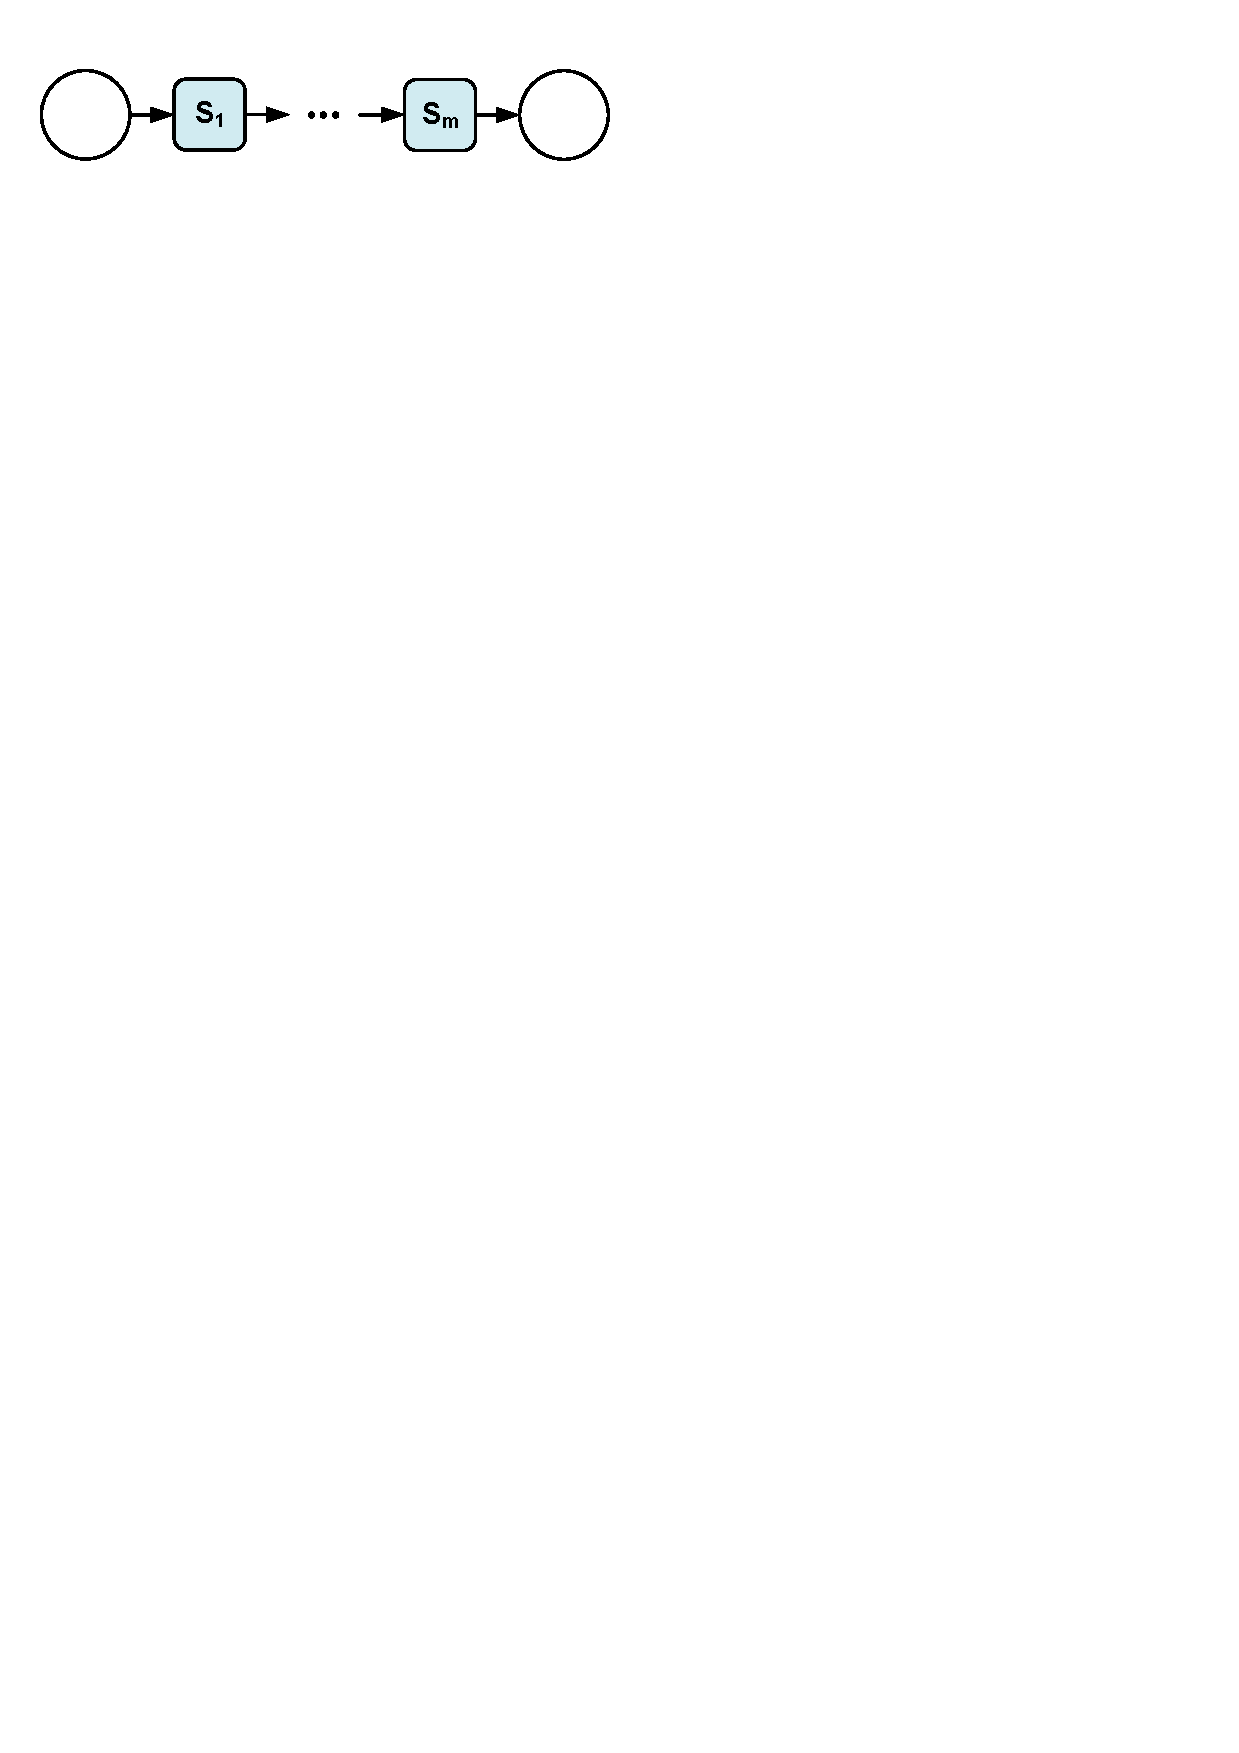
\includegraphics[width=1.8in]{sequence.pdf}\hfill\space\\[0.2cm]
$T=\sum\limits^m_{n=1}t_n$ \hfill $C=\sum\limits^m_{n=1}c_n$ \hfill
$A=\prod\limits^m_{n=1}a_n$ \hfill $R=\prod\limits^m_{n=1}r_n$
\end{tabular}}}
\caption{Sequence construct and calculation of its QoS
\cite{yu2013adaptive}.}
\label{sequence}
%\end{figure}
\vspace{0.3cm}
%\begin{figure}
\centerline{
\fbox{
\begin{tabular}{p{0.8\linewidth}}
\space\hfill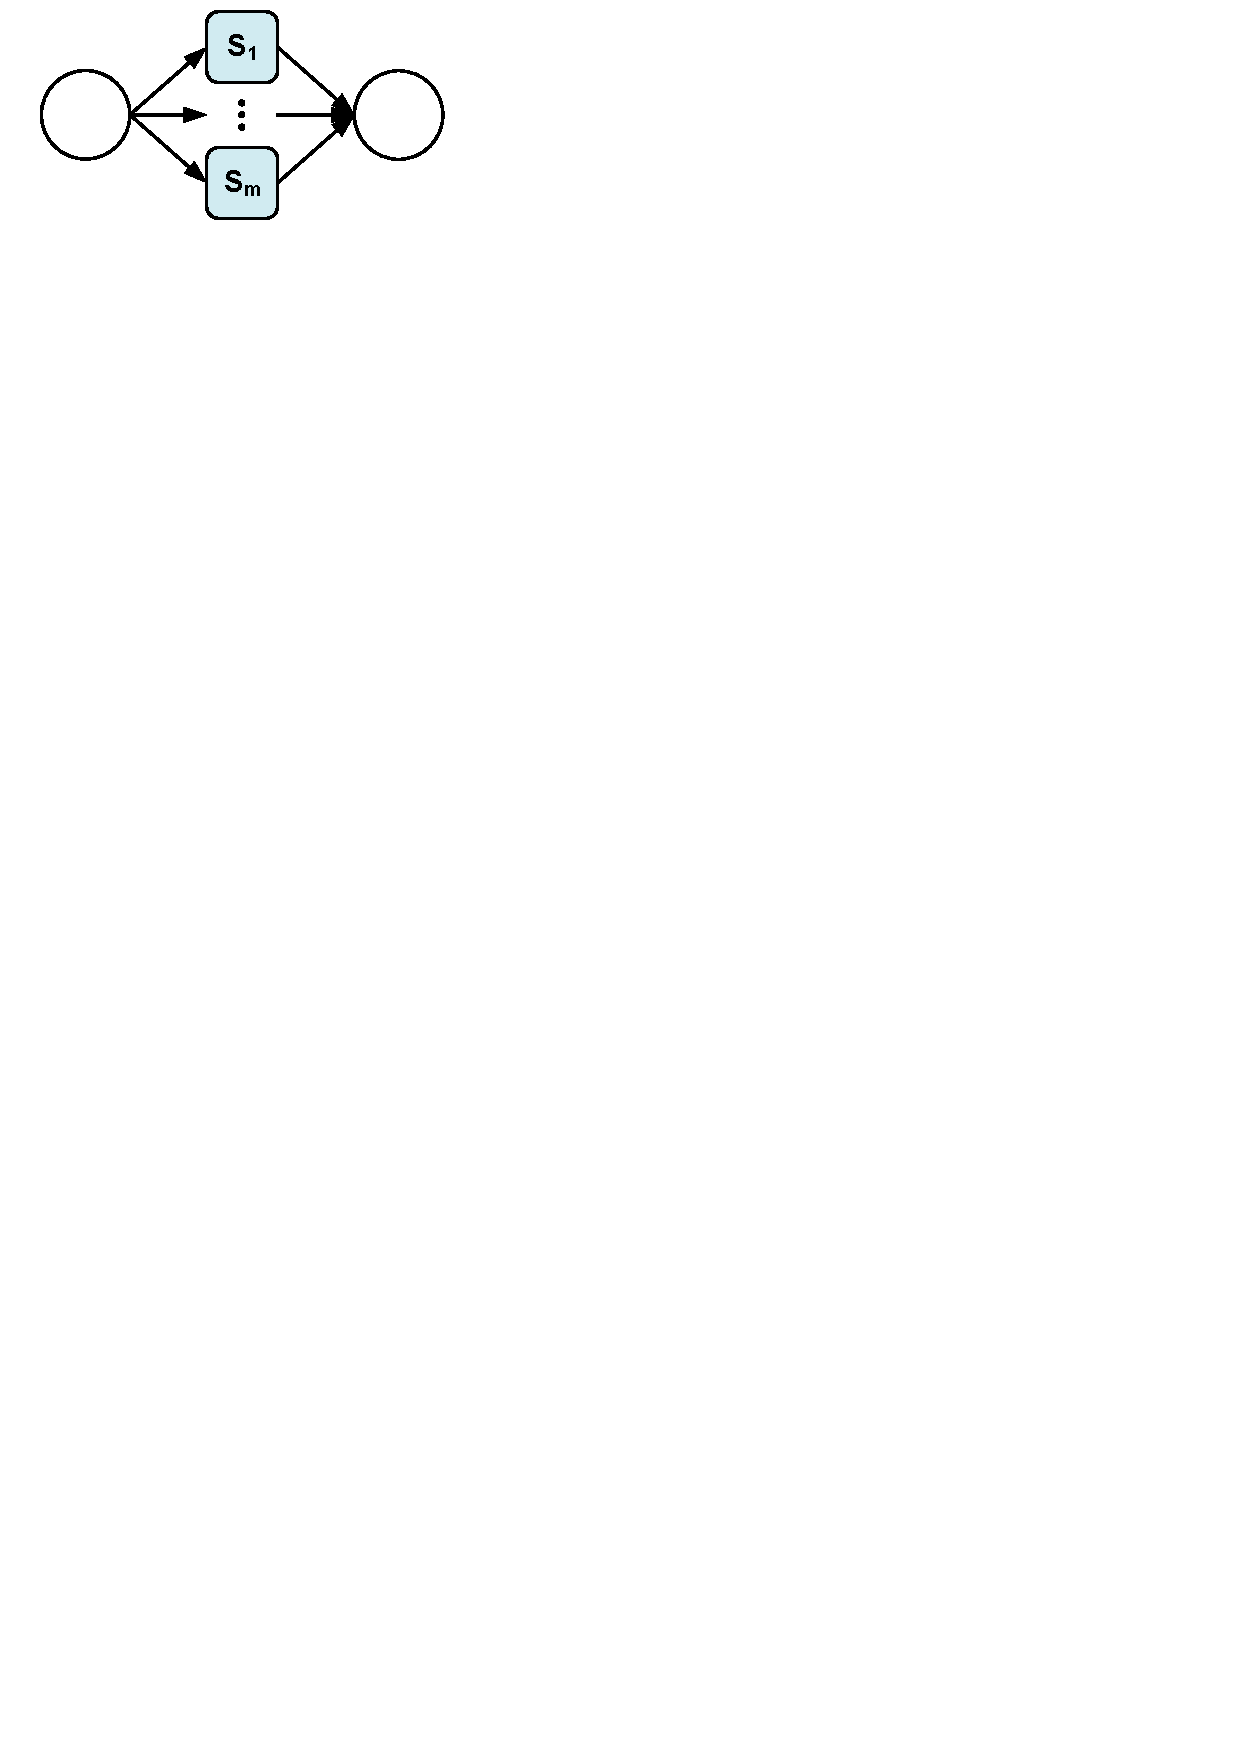
\includegraphics[width=1.4in]{parallel.pdf}\hfill\space\\[0.2cm]
\space\hfill$T=MAX\{t_n|n\in\{1,\ldots,m\}\}$\hfill\space\\[0.2cm]
$C=\sum\limits^m_{n=1}c_n$ \hfill $A=\prod\limits^m_{n=1}a_n$ \hfill
$R=\prod\limits^m_{n=1}r_n$
\end{tabular}}}
\caption{Parallel construct and calculation of its QoS
\cite{yu2013adaptive}.}
\label{parallel}
\centerline{
\fbox{
\begin{tabular}{p{0.8\linewidth}}
\space\hfill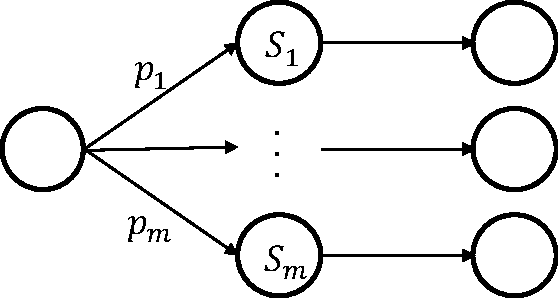
\includegraphics[width=1.4in]{choice.pdf}\hfill\space\\[0.2cm]
$T=\sum\limits^m_{n=1}p_n \cdot t_n$ \hfill $C=\sum\limits^m_{n=1}p_n \cdot c_n$ \hfill
$A=\prod\limits^m_{n=1}p_n \cdot a_n$ \hfill $R=\prod\limits^m_{n=1}p_n \cdot r_n$
\end{tabular}}}
\caption{Choice construct and calculation of its QoS
\cite{yu2013adaptive}.}
\label{choice}
\centerline{
\fbox{
\begin{tabular}{p{0.8\linewidth}}
\space\hfill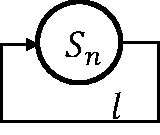
\includegraphics[width=1.4in]{loop.pdf}\hfill\space\\[0.2cm]
$T= \ell \cdot t$ \hfill $C=\ell \cdot c$ \hfill
$A=a^\ell$ \hfill $R=r^\ell$
\end{tabular}}}
\caption{Loop construct and calculation of its QoS
\cite{yu2013adaptive}.}
\label{loop}
\end{figure}

\subsection{Evolutionary Computation Techniques Overview}\label{ec}

Evolution Computing (EC) techniques are founded based on the principles of Darwin natural selection. The nature evolution and selection of individual in a population are automated simulated in EC techniques. In particular, a population of individuals is initialized for directly or indirectly presenting the solutions. Those individual candidates are evolved and evaluated using a fitness function to evaluate the degree of how good (or bad) of each individual. Therefore, it is possible to reach solution with near-optimal fitness. EC have been shown its promise in solving combinatorial optimization problems \cite{back1997evolutionary}. This is due to its flexibility in encoding the problems for the representation and its good performance in many scenarios. In particular, to manage the constraints in the problems, five main methods have been proposed deal with the constraints: coding, penalty functions, repair algorithm, indirect methods of representation and multi-objective optimization \cite{fleming2002evolutionary}. In the context of service composition. Many EC techniques have been approached for handling optimization problems for web service composition, such as Genetic Algorithms (GA) \cite{whitley1994genetic}, Genetic Programming (GP) \cite{koza1992genetic}, Particle Swarm Optimization (PSO) \cite{kennedy1995particle}, and Clonal Section Algorithm \cite{de2002learning}. These techniques are briefly introduced here.

GP is considered as a particular application of GA with a set of different encoded genes. In particular, the representation of GA is commonly represented as a linear structure. However, In GP, each individual is commonly represented as a tree structure. the tree structure has a terminal set and a function set, where variables, constants and functions are consisted of respectively. Also,  the tree structure is considered be efficiently evaluated recursively. Three genetic operators consisting of reproduction, crossover, and mutation are involved in to generate next generation for both GA and GP. Reproduction operator retains the elite individuals without any changes. Crossover operator replaces one node of one individual with another node of another individual. Mutation operator replaces a randomly selected node in an individual. The whole evaluation process won't stop unless an optimized solution found or a pre-defined number of generation reached.

PSO is one of swarm intelligence (SI) techniques that is based on the behavior of decentralized, self organized system. PSO algorithm is initialized by a group of random particles, which direct or indirect present the solutions. Those particles explores for the optimization position, which is approached by repeating the process of transferring particles position according to both their own best-known position and global best position.

Artificial immune system (AIS) has been studied for performing machine learning, pattern recognition and solving optimization problems.  Clonal Section Algorithm (CSA) is one of AIS for handling optimization problems, and the principle of utilizing Clonal Section Algorithm lie in the features of immune memory, affinity maturation. In particular, the antigen is considered as a fitness function instead of the explicit antigen population, and a proportion of antibody, rather than the best affinity antibody, are chosen to proliferation. Further more, speed and accuracy of the immune responses grow higher and higher after each infection even confronting cross-reactive response. Apart from that, hypermutation and receptor editing contribute to avoiding local optimization and selecting optimized solution respectively. 


\section{Related Work}\label{related}

\subsection{Single-Objective Web Service Composition Approaches}\label{singleobjective}

In this section, approaches to QoS-aware web service composition will be discussed in two distinct groups: EC-based approaches, which mainly rely on the EC techniques to reach the optimal solutions, and non-EC based methods, which do not utilize any bio-inspired methods. However, most of these approaches employ a single-objective fitness function for optimizing a united QoS score as a simple Additive Weighting (SAW) technique \cite{hwang1981lecture}.
\subsubsection{EC-based Composition Approaches}
EC-based web service composition mainly relies on evolutionary computation algorithms for searching optimal solutions. These algorithms are inspired by the behavior of human, animals or even T-cells. To use different EC algorithms, proper representations need to be designed. These representations directly or indirectly represent the service composition solutions. Herein we mainly discuss some promising research works on QoS-aware web service composition using  Genetic Algorithm (GA), Genetic Programming (GP), Particle Swarm optimization (PSO), and Clonal Selection Algorithm (CSA).

\textbf{Genetic Algorithm}. 
GA is a very reliable and powerful technique for solving combinatorial optimization problems \cite{srinivas1994genetic}. It has been applied to solve optimization problems for QoS-aware web service composition \cite{wang2012survey}. \cite{canfora2005approach} developed a GA-based approach for semi-automated QoS-aware service composition, where an abstract workflow is given. In their work, GA methods are compared to linear integer programming. The experimental finding reveals GA method is preferred when the size of service candidates are increasing.  \cite{tang2010hybrid} proposed a hybrid approach utilizing GA and local search. In particular, a local optimizer is developed and only recalled in the initial population for improving QoS value. This local search contributes to a better overall performance compared to GA-based methods without local search. In \cite{lecue2009optimizing},  a semi-automated service composition approach is developed in their paper for optimizing the quality of semantic matchmaking and some quality criteria of QoS. In particular, the quality of matchmaking problem is transferred to measure the quality of semantic links, which is proposed by two quality aspects: matchmaking type and degree of similarity.

\textbf{Genetic Programming}.
Tree-based representations could be more ideal for practical use, since they can present all composition constructs as inner nodes of trees. GP technique is utilised for handling tree-based representations. \cite {rodriguez2010composition} relies on GP utilizing a context-free grammar for population initialization, and uses a fitness function to penalize invalid individuals throughout evolutionary process. This method is considered to be less efficient as it represents a low rate of fitness convergence. To overcome the disadvantages of \cite {rodriguez2010composition}, \cite{yu2013adaptive} proposes a GP-based approach employing the standard GP to bypass the low rate of convergence and premature convergence. The idea of this paper is to increase the mutation rate while encountering low diversity in the population and adopt a higher crossover probability while trapped in local optimization.  During the evolutionary process, the elitism strategy is adopted, in which the best individual produced is reproduced to next generation directly without crossover and mutation. \cite{ma2015hybrid} proposes a hybrid approach combining GP and a greedy algorithm. In particular, a set of DAGs that represent valid solutions are initialised by a random greedy search and transferred into trees using the graph unfolding technique.  In each individual,  terminal nodes are considered as task inputs,  root node as  outputs, and all the inner nodes as atomic web services. During the reproduction process,  a randomly selected node on one individual is replaced with a new subtree generated by a greedy search to perform mutation while same atomic inner nodes in two random chosen individuals are swapped to perform crossover. However, \cite{da2016genetic} proposes a different transformation algorithm to present composition constructs as the functional nodes of trees. On the whole, all these GP-based approaches \cite{ma2015hybrid,rodriguez2010composition,da2016genetic,yu2013adaptive} consistenly ignore the semantic matchmaking quality, and their representations do not preserve semantic matchmaking information and composition constructs simultaneously. 

\textbf{Graph-Based Genetic Programming}.
A graph-evolutionary approach is introduced in \cite{da2015graphevol} with graph-based genetic operators, which is utilised to evolve graph-based representation. Although graph-based representations are capable of presenting all the matchmaking relationships as edges, they hardly present some composition constructs (e.g., loop and choice). Another paper \cite{da2016handling} investigated Directed Acyclic Graph with branches using GraphEvol approach \cite{da2015graphevol} to find near-optimal QoS solution in web service composition comparing with GP approach in \cite{da2015gp}. The experiment results reveal a significant improvement in execution time while slightly tradeoff in the fitness value. However, the service composition problem for handling branches is not generally formulated, i.e., only works for one choice construct. If more one nested choice constructs, their approach does not work any more.

\textbf{Particle Swarm optimization}.
PSO is considered to a simple and effective approach for solving combinatorial optimization problems with few parameters settings \cite{long2009environment}. The paper \cite{long2009environment} proposed an environmental-aware PSO approach for QoS-aware web service composition. In particular, an improved discrete PSO algorithm is developed for adapting the changes of composition environment (i.e., services) when a same service composition request is called more than one time. The paper \cite{liu2007hybrid} proposed a hybrid Genetic Particle Swarm optimization Algorithm (GPSA). In their work, GA is employed with only crossover operator to produce new individuals with $n_1$ iterations while PSO is only utilized for local searching (i.e., $C_2$ parameter is set to 0 in the standard velocity updating functional) with $n_2$ iterations. This approach achieves a good balance of global and local optimization through a  mechanism based on two thresholds, which determine the values of $n_1$ and $n_2$. However, these works \cite{liu2007hybrid,long2009environment} handle only semi-automated service composition problems. On the other hand, \cite{da2016particle} proposes a PSO-based fully automated approach to generate a composition graph from a queue. The idea is to translate the particle location into a service queue as an indirect representation of composition  graph, so finding the best fitness of the composite graph is to discover the optimized location of the particle in the search space. \cite{da2016particle} proposes a PSO-based fully automated approach to generate a composition graph from an indirect representation, i.e., a service queue. This service queue is mapped to particles' locations, so finding the best fitness of the composite graph is to discover the optimized location of the particle in the search space. In particular,  the dimension of the particle is set up as the same number as relevant web services, and the index of services is mapped to the location vectors in a particle and put services in a queue in ascending order, from which a graph is decoded using a forward GraphPlan Algorithm. However, These fully automated approaches only optimize QoS.

\textbf{Clonal Selection Algorithm}.
The paper \cite{yan2006immune} introduces a novel web service composition approach using an immune algorithm for global optimization considering optimum time under a constraint on cost. As a given abstract graph could be broken into several single pipelines, the optimization problem is transferred into getting the optimum executing plan for the single pipelines. In a pipeline, each involved tasked could be slotted with several alternative web services with QoS values labelled to their edges so that a weighted multistage graph is established for a longest path selection. In the immune algorithm, the service composition problem is encoded using a binary string as an antibody for evaluating the affinity value regarding the antigen ( fitness function ), and the antibody with low concentration will be selected in a high probability of crossover and mutation for new antibody generation. However, the efficiency of creating the weighted multistage graph would be considered to be less efficient. The paper \cite{pop2009immune} introduced an immune-inspired web service composition approach combining an enhancing planning graph (EPG) and a clonal selection algorithm to solve optimization problem considering both semantic link quality and QoS.  The EPG model is characterized with action and layer involved in multiple stages, where each action represents clustered web service, and each layer represents input or output parameters grouped in concepts.   During the clonal selection process, the antigen is represented as a fitness function, and the antibody is represented as a binary alphabet to encode EPG.  The remaining steps are standard computation procedure for CLONALG, which consists of clones generation from selected antibody, affinity maturation process, low-affinity antibody replacement. We re-select antibody and repeat all the procedure. At last, the approach is proved to reach an optimal solution or a near-optimal solution in the experiments under trip and social event attendance planning domains.

\subsubsection{AI Based Approaches}

AI Planning techniques have been widely employed for service composition \cite{markou2015non,peer2005web}. The main idea of these techniques considers services as actions that are defined with functional properties ( i.e., inputs, outputs, preconditions and effects) to generate validate service compositions using classic planning algorithms. 

Various AI planning approaches \cite{feng2013dynamic,huang2009effective,rao2006mixed,wang2013genetic, wang2014automated} have been presented to solve semantic web service composition problems using the Graphplan \cite{blum1997fast} algorithm. \cite{wang2014automated} employs the Graphplan to secure the correctness of overall functionality, which enables atomic web services to be concretely selected and accurately matched for achieving desired functionality. In particular, conditional branch structure is also correctly handled. The pitfalls of this approach are procuring only linear sequences of actions, and it is hard to deal with QoS optimization. In paper \cite{feng2013dynamic}, service-dependent QoS is modeled and considered for QoS-aware web service composition. This dependent QoS model is formed in three cases: a default QoS attribute, a partially dependent QoS attribute, and a completely dependent QoS attribute, and they are used for the dependency checking base on a backwards Graph building with a breadth-first strategy. However, computation of service dependencies is very intensive for initialization and updating. Some approaches \cite{lecue2007making,sohrabi2009web} rely some frameworks supported by particular agent programming languages (e.g., Golog \cite{sohrabi2009web}  and SHOP2 \cite{sirin2004htn}) to composite web services. In \cite{sohrabi2009web}, a service composition framework supported by Golog. Golog is used to present the generic procedure, and situation calculus and first order language (FOL) are used to describe the properties of services and users' preferences. Therefore, Golog can effectively perform a constant search to reach a terminating situation as a service composition solution. As summarized here, given the desired solutions generated to meet users' complex requirements, AI planning techniques are considered to be less efficient, and not capable of dealing with optimization solutions for service composition (e.g., generate either optimal QoS or number of services ) independently. In addition, they may suffer scalability issues when large repositories are given. 

\subsubsection{Other Approaches}
The non-EC based approaches do not rely on bio-inspired approaches. They target the optimized service composition solutions by some other methods. For example, integer programming, exhaustive search, local search and so on.

\textbf{Integer Linear Programming (ILP)}. ILP methods are utilized for achieving web service composition. Generally, an ILP model is created with three inputs provided: a set of decision variables, an objective function and a set of constraints. On the other hand, the outputs are maximized/minimize objective function and values of decision variables. Therefore, ILP is flexible in taking QoS into account, handling constraints for QoS and optimizing the objective function for QoS-aware service composition problem. \cite{gao2005web} define a zero-one IP model for web service composition based on an abstract service workflow, where services may be different in QoS, but classified into the same classes.  \cite{yoo2008web} formulated web service composition problem based on the model introduced in \cite{gao2005web}. Apart from that, compared with the previous work, they simultaneously take both QoS and constraints on QoS into account. However, on the one hand, due to the increase in the number of decision variables, ILP may lead to exponentially increase the complexity and cost in computation \cite{li2016full}. The resulted huge delay is not allowed in the real world scenarios. In addition, if non-linear function is utilized, the scalability is a big problem.
 
\textbf{Dynamic Programming Approach}. Dynamic programming is an effective method for solving problems, where many repetitions of their break-down subproblems and optimal substructures are presented. In  \cite{huang2009effective}, an efficient pruning approach is developed including a forward filtering algorithm for searching task related service candidates, a modified dynamic programming approach for dealing a subproblem of service composition (i.e., a  problem on satisfaction of each concept pool of each graph layer ), and a backward-search method for searching optimal composition results. This paper \cite{xu2012towards} forges a problem to solve large-scale service composition efficiently with QoS guarantee, where a dynamic programming algorithm named QDA is developed to for ensuring the optimization of the composition problem. The optimization problem is solved by optimizing every subproblem based consideration of web service composition with fewest services involved in.  In particularly, best-known QoS are recorded and updated for all added web services, and service parameters by the maximum of the path using the traceback depth-first search to derive an execution plan. However, the global best QoS could be never reached since a trade-off in the efficiency of QoS guarantee in solutions.

\textbf{ER Model-Based Approach (ILP)}. Most of the small and medium business rely on ER database to process information and data. \cite{xu2010semantic} employs ER model to construct domain ontology and semantic web services.  It potentially benefits large groups of organizations. With regard to the ontology construction, it realizes the transformation from ER to OWL-DL, which has maximum expressiveness while retaining computational completeness and decidability. Also,  it constructs semantic web service described by OWL-S  from ER.  Therefore, the semantic web service composition problem is transferred to reason composite service based on a link path between entities in the ER model corresponding to the classes.  However, other constructs such as loop and switch constructs cannot be effectively expressed in their approach, which demands many further research. They do not consider optimization problem at all.

\subsection{Multi-objective, and Many-objective Web Service Composition Approaches}\label{multiobjective}
%----------------------chen starts---------------------------------------------------
Maximizing or minimizing a single objective function is a most commonly used way to handle optimizing problems in automated web service composition.  That is a Simple Additive Weighting (SAW) \cite{hwang1981lecture} technique, which presents a utility function for all the individual quality criteria as a whole. This technique optimizes and ranks each web service composition using a single value for each solution. However,  the limitation of this technique lies in not handing the conflicting quality criteria.  Those conflicting quality criteria are always presented trade-offs. To overcome this limitation, a set of objectives corresponding to different independent quality criteria are optimized simultaneously. Consequently,  a set of promising solutions that presents many quality criteria trade-offs are returned.


\subsubsection{Multi-objective approaches}\label{MultiObjective}

Many multi-objective techniques \cite{liu2005dynamic,zhang2010qos,yu2013efficient,yin2014hybrid,xiang2014qos,chen2014partial} have been investigated to extensively study QoS-aware web service composition problems.  A set of optimized solutions is ranked based on a set of independent objectives, i.e., different QoS attributes. In particular, solutions are compared according to their relationship for domination. That is, figure out solutions that clearly dominate the others. For example, given two service composition solutions that are compared based on execution cost $c$ and execution time $t$, solution one, $wsc_1(c=10,t=1)$ and solution two,  $wsc_2(c=13,t=1)$. In our context, $wsc_1$ dominate $wsc_2$ as $wsc_1$ has the same execution time and a lower execution cost. If given $wsc_3(c=10,t=2)$, $wsc_2$ is a \textit{non-dominant} solution in the relation to $wsc_3$ because of its longer execution time and cheaper execution cost. Therefore,  If those non-dominant solutions are globally produced among both the dominant and non-dominant solutions, i.e., they do not dominate themselves. These solutions are called a \textit{Pareto Front}, which provide a set of non-dominant solutions for users to choose.


\textbf{Multi-objective techniques with GA} Many approaches to multi-objective web service composition employs GA \cite{liu2005dynamic}, but other EC algorithms are also considered. For GA, \cite{liu2005dynamic} employs a service composition model, called  MCOOP (i.e., multi-constraint and multi-objective optimal path) as web service composition solution, where only a sequence composition construct is considered in the paper. In this model, different paths are selected from a service composition graph that includes $N$ service group. In each group,  services present same functionality with different QoS.  Apart from that, GPDSS is proposed to generate the outputs of Pareto optimal composition paths. In particular, two points crossover and mutation are applied to speed up the astringency of this algorithm. The work \cite{wada2012e3} investigates a semi-automated approach to SLA-aware web service composition problem.  Each linear representation presents three service composition solutions designed for three group users' categories.  The individuals are randomly initialized, evaluated and optimized with objectives from all the possible combinations of throughput, latency, cost and user category.  In this work, two multi-objective genetic algorithms: E-MOGA and Extreme-E are developed. E-MOGA is proposed to search a set of solutions that equally distributed in the searching space by the means of fitness function, where the production of domination value,  Manhattan distance to the worst point and sparsity (i.e, Manhattan distance to the closest neighbor individual)  is assigned to the feasible individual as fitness value, and SLA violation /domination value is assigned to the infeasible solutions. On the other hand, Extrem-E provide extreme solutions by employing fitness functional, where weights use a term 1/exp(p-1), where $p$ is the number of objectives and is assigned to the $p^{th}$ objective.

\textbf{Multi-objective techniques with PSO} The work \cite{yin2014hybrid} combines genetic operators and particle swarm optimization algorithm together to tackle the multi-objective SLA-aware web service composition problems. The method proposed in the paper  is considered to be more effective for  considering different scare of cases.  It is called as HMDPSO, i.e., hybrid multi-objective discrete particle swarm optimization. In particular, the updates of particle's velocity and position are achieved by the crossover operator, where both velocity and position of new individual are updated in accordance with positions of \textit{pbest}, \textit{gbest}, and current velocity. On the other hand, mutation strategy is introduced to increase the diversity of particle, and it perform on the \textit{gbest} particle if the proposed swarm diversity indicator is below some value. For the evaluation,  the fitness values of individuals are assigned in the same way as the E-MOGA method in \cite{wada2012e3}.

\textbf{Multi-objective techniques with ACO} Generally, ACO simulates foraging behaviors of a group of ants for optimizing the traversed foraging path, where the strength of pheromones is taken account for. The work \cite{zhang2010qos} turns the service composition problem into path selection problem for a given abstract workflow with different service candidate sets. It employs a different strategy of "divide and conquer`` for decomposing a given workflow. That is,  two or more abstract execution paths are decomposed from the workflow and have no overlapped abstract services. This decomposing strategy results in a much smaller length of the execution paths compared to those in the works \cite{yu2007efficient}.  Also, a new ACO algorithm is proposed to handle the multi-objective QoS-aware service composition problem. In particular,  the phenomenon is presented as a k-tuple for $k$ objectives, rather than a single value. Apart from that, a different phenomenon updating rule is proposed by considering an employment of a proposed utility function as a global criterion. The paper \cite{wang2014novel} introduces nonfunctional attributes of web services to include trust degree according to the execution log. Also, a novel adaptive ant colony optimization algorithm is proposed to overcome the slow convergence presented from the traditional ant colony optimization algorithm. In particular, the pheromone strength coefficient is adjusted dynamically to control both the updating and evaporation of pheromone. The experiment results are analysed in an alternative way. That is, the total Pareto solutions are combined from different compared ACO algorithms, then the accurate rate of each algorithm is calculated based on the compared Pareto solutions identified in the total Pareto solutions. The results also show more Pareto solutions found compared to the traditional ACO methods. However, the experiment is only conducted for the evaluation of a small case study, where only a simple abstract workflow is studied.

\subsubsection{Many-objective approaches}\label{ManyObjective}

Herein, more than three objectives in multi-objective problems (MOPs) are often considered as many-objective problems. Ishibuchi et al. \cite{ishibuchi2008evolutionary} present an analysis of the multi-objective algorithm for handling optimization problems with more than 3 objectives. However, they address that the searching ability is deteriorating while the number of objectives is increasing, since the non-dominated solution is very large, which make it harder to move solutions towards the Pareto Front.

The work \cite{de2010many} employs NSGA-II to deal with five different quality criteria (i.e., runtime, price, reputation, availability and reliability) for semi-automated web service composition problem.  To examine the techniques to decrease the deterioration, two preference relations proposed by \cite{bentley1997finding} are applied to NSGA-II: Maximum Ranking (MR) and Average Ranking methods (AR). In particular, MR is the best of all the ranking scores from all the objectives, and AR is a sum of all the ranking scores from all the objectives. Therefore, three algorithms (NSGA-II, NSGA-II with MR and NSGA-II with AR) are evaluated for studying the five different performance metrics ( i.e., hypervolume \cite{zitzler1999evolutionary}, Generational Distance \cite{van2000measuring}, Spread and Coverage \cite{zitzler2000comparison}, and pseudo Pareto front (i.e, a combination of all non-dominated solutions)),  where An empirical evaluation is performed on. The experiment shows NSGA-II with AR outperforms others in both GD and Spread (i.e., more balanced solutions). However,  a certain region of  Pareto Front is generated by NSGA-II,  rather than a wider distribution for the solutions. NSGA-II with MR performs intermediately compared to the other two algorithms. On the whole,  this work, for the first time, takes two preference relations into account for solving many-objective service composition problem, and contribute to finding better solutions with many performance metrics.



\subsubsection{Preferences Articulation Techniques for Multi-and Many-objective Approaches}\label{PreferencesMultiObjective}
Most of the EMO algorithms focus on generating evenly distributed non-dominated Pareto solutions. Often, an indispensable decision must be made for choosing a small number of solutions, which satisfy customers' preferences. However, in some practical scenarios, some issues in EMO algorithms need to be handled when no or few solutions are gained in the preferred areas or far-optimal solutions are gained. To solve these issues, some user preferences-based approaches have been proposed to search only the space that preferred by users and to increases the density of solutions in that space. These approaches can be classified into three groups based on the articulation of preferences \cite{van2000multiobjective}. The first group is prior approaches, where the articulation is done before optimization process; The second group is interactive approaches, where the articulation is done during optimization process; The third group is posteriori approaches, where the articulation is done after optimization process. As argued in \cite{giagkiozis2014pareto}, the third approaches are capable of generating more desired solutions in the preferred region. 


Most of the multi-objective service composition assumes that the user preferences are not known in advance. However,  often, a vague preference is provided by users at least, and preferred solutions are roughly specified by them.  These vague preferences should be taken into decision making and could guide us in searching the most interesting areas on the Pareto front in a more effective and efficient way. In \cite{branke2005integrating}, they proposed two effective and efficient methods for finding the most relevant parts of Pareto solutions according to users' preferences. In particular, vague trade-offs between different objectives are taken into account when users have some rough thoughts about trade-offs.  The first method is based on a guided multi-objective evolutionary algorithm in \cite{branke2001guidance}, and the second one is approached by a new biased crowding operator. In the first method, the dominance is specified for the maximally acceptable trade-offs of each pair of objectives, and the space of objectives is appropriately transferred into two auxiliary objectives. The second method works on finding a biased distribution on the Pareto solutions. The idea of this method is to introduce a biased crowding distance, which controls the expansion of solutions according to their location projected on a proposed hyper plane, i.e., users' specified direction vector.  The experiment conducted shows that two methods achieve an effective and efficient way of finding relevant Pareto solutions for users. In \cite{cheng2015reference}, a posteriori articulation method is proposed to find Pareto solutions in the preferred areas. In particular, reference vectors are utilised by a decision maker according to users' preferences. The reference vectors can be easily defined either in a priori or a posterior. In their paper, a posteriori is adopted based on the observation of given Pareto solutions. The reference vectors divide the objective space into subspaces, where one individual is selected from each subspace and put into the next generation. Therefore, the newly generated individuals move towards optimal Pareto Front and reference vectors. The experiments show that this method could handle preferences effectively and efficiently as well as more optimal Pareto solutions found. On the whole, none of existing preference articulation techniques focus on web service composition, let alone applicability for comprehensive quality-aware semantic web service composition. 



\subsection{Dynamic Web Service Composition Approaches}\label{dynamicserivce}
All the previously discussed approaches can be classified into one group that assumes the composition environment is static. The rest approaches can be classified into another group that does not make that closed world assumption. Instead, a real world scenario taken a dynamic composition environment into account. For example, nonfunctional properties of web services may fluctuate over time or services are failed/newly registered. A few researcher works on the second group to cope with the dynamic composition environment. To address this problem \cite{nasridinov2012qos},  a suitable mechanism for effectively and efficiently handle this problem raise a significant challenge for the practical value.

\subsubsection{Dynamic Web Service Composition Approaches For Changes in QoS}\label{dynamicQoS}

Service selection is one of the crucial steps when we compose services. In the context of static web service composition, we always selection services based on the QoS advertised by service providers. However, QoS is fluctuating over the time. The executed instances of a service for the run time indicate a real QoS value. This dynamic QoS is formally modeled as an uncertain QoS model.  Based on this model, some studied \cite{wen2014probabilistic} has been addressed recently. In \cite{wen2014probabilistic}, the QoS model describes the probabilities of different dominating relationships in the instances of all services within the same class. To efficient provide a relatively small set of services for selection that is based on the uncertain QoS model, the data structure of R-tree is introduced for spatial query on multidimensional data (i.e., many dimension of QoS attributes) since it can significantly reduce the searching space. This space index technique is one of the key contributions in this paper for efficiently store and retrieve services for service selection. 

Reinforcement learning (RL) is one technique of machine learning for solving sequential decision-making problems to maximize some long-term rewards.  RL is utilized to deal with how actions are taken in an uncertain environment. In our context, this uncertain environment is related to QoS. In \cite{mostafa2015multi}, they combines multi-objective optimization and reinforcement techniques to solve multi-objective service composition problem in an uncertain and dynamic environment. In particular, we service composition is modeled based on Partially Observable Markov Decision Process (POMDP), and solutions to services composition are considered to be a set of decision policies. Each of the decision policies is considered as a procedure of service selection (i.e., a single workflow). They proposed approach in this paper to learn an optimal selection policy. 

\subsubsection{Dynamic Web Service Composition Approaches For Service Failure}\label{dynamicService}
Traditionally, re-selection of failed service is one of widely used approach to re-ensure the desired execution web service composition. The idea of this traditional approach restores many alternative service candidates for each component service involved in the composition solution. If component service confronts failure, the alternatives are used for the replacement.  A framework, WS-Replication is introduced in \cite{salas2006ws}, which mainly address service failure using the idea of the traditional method. \cite{yin2010qos} further introduce a more complicated model that address attributes of not only QoS but also transactionality for more reliable replacement. However, those approaches \cite{salas2006ws,yin2010qos} have a huge cost in computation due to the re-selection mechanisms \cite{nasridinov2012qos}. To overcome the disadvantage of traditional resection approach, \cite{nasridinov2012qos} proposes a QoS-aware performance prediction for self-healing web service composition system. This system consists of three main phases: monitoring, diagnosis and repair. The monitoring phase is to detect degradation, diagnosis is to identify the source of degradation, and repair is to reselect desired services. To minimising the number of re-selection in the phase of repair, decision tree learning is used to the prediction of the performance based on the QoS. This technique outperforms other classification techniques (i.e., back propagation neural network, support vector machine probabilistic neural network, and group method of data handling and regression tree) by accuracy in \cite{mohanty2010web}.  Those works mainly focus on services failure, and they do not recognise the importance of  QoS changes of service in the repository. \cite{wagner2016robust} proposes a method to cluster services that are back up for service failure. This method determines a set of backup services based on their functional properties for service repairing. By employing functional properties, services and their combinable services are identified. The fragmented clusters are formed based on the subsume relationship among their associated combinable services. Also, to merge these fragmented clusters, unified clusters are created by adding virtual services that subsume the fragmented clusters. Therefore, a set of backup services is provided in both the clusters that the failure services involved in and their sub-clusters, from which we could select suitable service.


\subsection{Semantic Web Service Composition Approaches}\label{Semantic}
Sophisticated real-world applications demand complex requirements in developing service composition. Apart from consideration of both the functional and nonfunctional properties of web services, more complex chaining strategies of semantic services are necessarily arranged to satisfy dependency constraints in the real world. To cope with these complicated requirements, preconditions and effects are semantically described using logic formula to enable the complex service composition. Many standards have been established for supporting the chaining ability of semantic web services, such as OWL-S. OWL-S accommodates varieties of structural constructs for service composition, namely: Sequence, Unordered, Choice, If-Then-Else, Iterate, Repeat-While, Repeat-Until, Split and ``Split + Join'' \cite{wang2014automated}. For example, ``Split+Join'' calls for the process consisting of the parallel execution of a collection of process components with barrier synchronization. That is, ``Split+Join'' doesn't completes until all of its components processes have been completed. Additionally, ``Split'' and ``Split+Join'' can be applied for partial synchronization \cite{wang2014automated}.

Most of the existing service composition approaches do not fully consider services associated with preconditions and effects. Therefore, it is hard to generate service composition solutions with branch structure in a fully automated way. The importance of preconditions and effects are ignored that specifies preconditions needed to be satisfied and effects resulted from service execution. The execution of these services could causes side effects in the world. However, some approaches do consider preconditions and effects using classic AI planning methods. The limitation of these approaches lies in the linear sequences of actions.


A generalized semantic web service composition is introduced in \cite{bansal2016generalized}, preconditions and effects are effectively presented in a conditional directed acyclic graph where conditional nodes created with two outgoing edges representing the satisfied and the unsatisfied case at the run time. They filter the solutions based on the trust rate using Centrality Measure of Social Networks to find web service trusted by the customers. They also implement semantic web service composition engine for automated conditional service composition. The main limitation of this work is that the loops structure are not considered in their web service representation, and they leave optimization problems aside.

This paper \cite{wang2016automatic}  addresses a critical problem by considering services with preconditions and effects. In a real world scenario, this problem can significantly affect service composition solutions.  In their paper, an extensive Graphplan technique is proposed to support the representation of the problem with execution effects. In particular, a two-level directed graph, called planning graph (PG) is utilized and comprises of two kinds of nodes (proposition and action ones) and three kinds of edges (precondition-edges, add-edges, and delete-edges). The proposition and action level is alternated between each other in the PG.  By utilizing this presentation, the branch structure is supported in the service composition solution when some uncertain effects are produced by some services. 

\subsection{Summary and Limitations}\label{summary}

An overview of recent related research on web service composition is presented in this chapter. The first related research discussed is \textbf{single-objective web service composition approaches}, which mainly works on generating composition solutions with optimal QoS or number of services based on the objective functions. On the one hand, EC-based approaches have been widely used for effectively and efficiently solving the above problems. On the other hand, non-EC based approaches, such as AI planning approaches, Integer Linear Programming, Dynamic Programming Approaches are employed in web service composition, but they may suffer scalability due to the increase in complexity of the problem or leave aside optimization problem. The key limitation of single-objective web service composition approaches is that the importance of semantic matchmaking quality is ignored, which should be simultaneously taken into account with QoS. To cover this necessity, new representations and quality model must be proposed along with service composition methods.

The second related research area discussed is \textbf{multi-objective, and many-objective composition approaches}, in which different independent quality criteria of QoS are separately optimized and a set of solutions is produced.  These solutions present different tradeoffs among different quality criteria of QoS. Multi-objective composition approaches optimize two or three independently quality criteria, while many-objective composition approaches optimize more than three quality criteria. One limitation of multi-objective or many objectives approaches is that one important quality criteria, i.e., quality of semantic matchmaking, is not considered. Apart from that,  constraints on both SLA and quality of semantic matchmaking are not simultaneously taken into account. Meanwhile, none of existing preference articulation techniques focus on web service composition problems. Therefore, it is very interesting and challenging to simultaneously to take these interesting problems into account.

\textbf{Dynamic web service composition approaches} are discussed in the third related research area, where a closed world assumption is dropped. In particular, the composition environment is changing over time, which gives birth to two dynamic service composition problems. One is related to the changes in QoS, and another is to the changes in the availability of services. Existing dynamic web service composition mainly works on service selection using non-EC techniques. These techniques aim to adapt the changes in the solutions, such as re-selection of changed services. However, the cost of initial planning is consistently ignored and separated from the adaption of a dynamic environment. In addition, some interesting problems are not taken into account, such as the changes of ontology that is utilized to describe the functional properties of services,  and new service may register in the services repository.

The last related research area focuses on \textbf{semantic web service composition approaches}, which explore a more complex and realistic service composition. Most of existing semantic web service composition is merely based on the inputs and outputs of services, Beside these functional properties,  precondition and effects are occasionally considered when they compose services. However,   The support for preconditions and effects is not fully investigated along with global optimization in existing works since they potentially bring various of composition constructs into consideration. Achieving semantic service composition considering all these composition constructs and global optimization on a comprehensive quality is a big challenge.

